\chapter*{3 Versuchsdurchführung und Auswertung}
\addcontentsline{toc}{chapter}{3 Versuchsdurchführung und Auswertung}
\setcounter{chapter}{3}
\setcounter{section}{0}
\setcounter{subsection}{0}
\vspace{-2em}
\section{Versuch 1 - Signaldarstellung mit dem Analog-Oszilloskop}
\vspace{-1em}
    \subsection{Versuchsaufbau und -durchführung}
    Zunächst wurde uns ein Signal vom Betreuer vorgegeben, welches wir mit dem Oszilloskop untersuchen sollten. Diese ist für uns von unbekannter Form, Frequenz und Amplitude. Wir haben uns dann für folgende Einstellung am Oszilloskop entschieden:
   
    Time/Div: 5$\mu$s 
    Volt/Div: 0.5 V
   
    $\Rightarrow$ Die Amplitude $U_0$ des Signals ist 1.2 V und die Periodendauer 45 $\mu$s. Die Frequenz des Signals ist dann:
    \vspace{-0.5em}
    \begin{equation}
        f = \frac{1}{T} = \frac{1}{45\mu s} = 21.7 kHz
        \label{eq:Versuch1_Frequenz}
    \end{equation}
    \vspace{-0.5em}
    Das Schirmbild sah wie folgt aus:
    \begin{figure}[H]
        \centering
        \caption{Schirmbild des vorgegebenen Signals}
        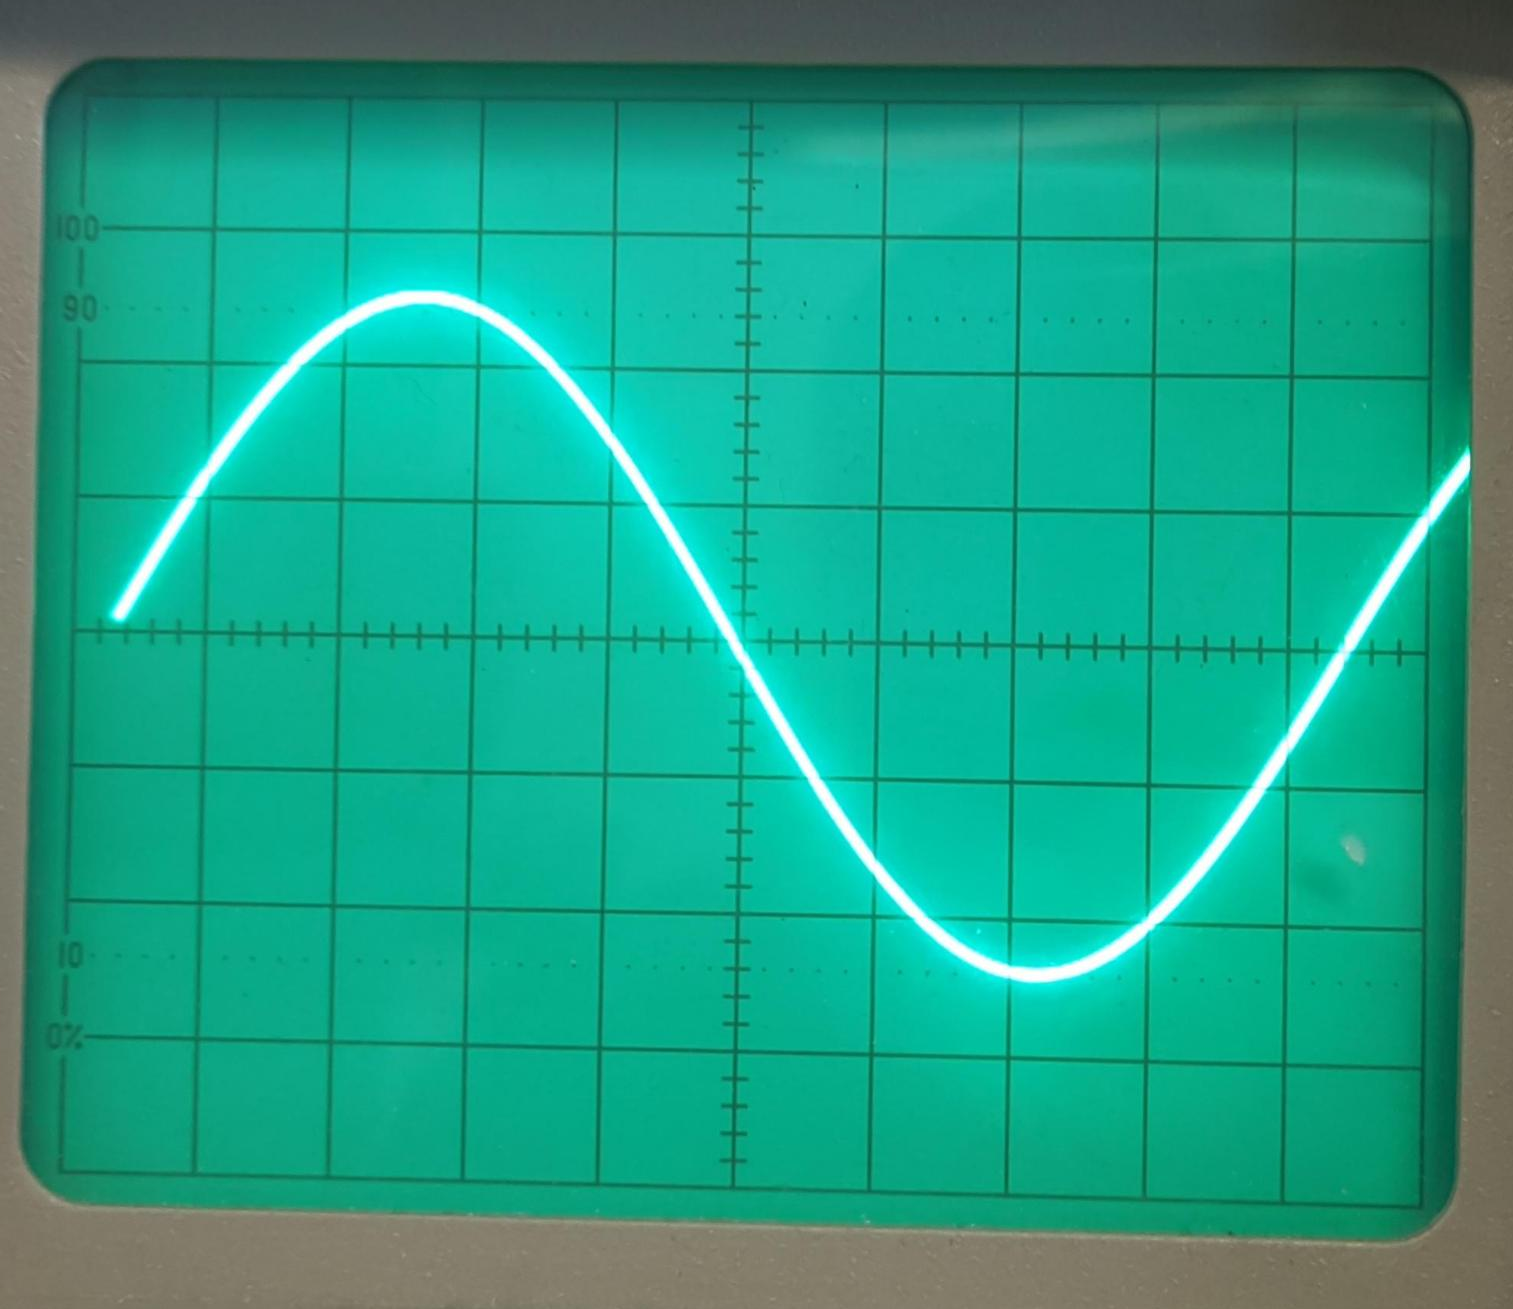
\includegraphics[width=0.8\textwidth]{bilder/Versuch_1.png}
        \label{fig:Versuch1_Schirmbild}
    \end{figure}

    Nun können wir folgende Messwerte ablesen:
    \begin{table}[H]
        \centering
        \caption{Messwerte des vorgegebenen Signals}
        \vspace{0.5em}
        \begin{tabular}{|c|c|}
            \hline
            \textbf{Größe} & \textbf{Wert} \\
            \hline
            Amplitude $U_0$ & 1.2 V $\pm$ 0.5 V \\
            \hline
            Frequenz & 21.7 kHz $\pm$ 0.1 kHz\\
            \hline
            Periodendauer & 45 $\mu$s $\pm$ 5 $\mu$s \\
            \hline
        \end{tabular}
        
        \label{tab:Versuch1_Messwerte}
    \end{table}
    
    Wir können nun mit folgender Formel die Frequenz des Signals berechnen:

    \begin{equation}
        f = \frac{1}{T}
        \label{eq:Versuch1_Frequenz}
    \end{equation}

    Und den Größtfehler mit folgender Formel berechnen:

    \begin{equation}
        \begin{aligned}
            \Delta f = \left |\frac{1}{T^2} \right | \cdot \Delta T \\
            \Rightarrow f^2 \cdot \Delta T
        \label{eq:Versuch1_Frequenz_Fehler}
        \end{aligned}
    \end{equation}
        
    Der Größtfehler der Frequenz beträgt nach \ref{eq:Versuch1_Frequenz_Fehler} 0.1 kHz. Die Frequenz des Signals beträgt also 21.7 kHz $\pm$ 0.1 kHz. \textcolor{red}{TODO: REchnung prüfen}
    
    \subsection{Ergebnisse}
    \textcolor{red}{TODO}


\section{Versuch 2 - Impedanzmessung an Widerstand, Kondensator und Spule}
    
    \subsection{Versuchsaufbau und -durchführung}
    \begin{figure}[H]
        \centering
        \caption{Schaltbild Versuch 2}
        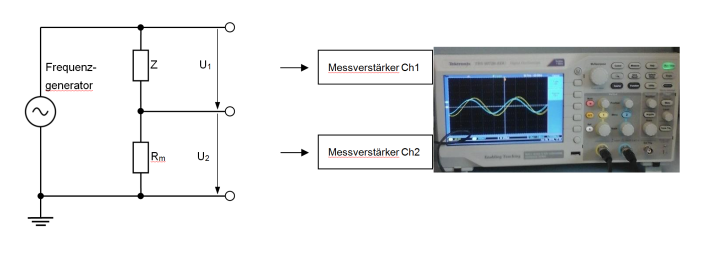
\includegraphics[width=\textwidth]{bilder/Versuch2_Aufbau.png}
        \label{fig:Versuch2_Schaltbild}
    \end{figure}

    \textcolor{red}{TODO: Fehler mit angeben. Skala war 200mV/Div}
    Nun lässt sich aus dem Aufbau \ref{fig:Versuch2_Schaltbild} noch der Widerstand Z berechnen. Da gilt: 

    \begin{equation}
        \begin{aligned}
            \frac{U_m}{U_z} = \frac{R_m}{|Z|} \\
            \Rightarrow |Z| = \frac{U_z}{U_m} \cdot R_m
            \label{eq:Versuch2_Impedanz}
        \end{aligned}
    \end{equation}
    |Z| ist nach \ref{eq:Versuch2_Impedanz} 99.82 $\Omega$. Der Größtfehler beträgt:
    \begin{equation}
        \begin{aligned}
            \Delta |Z| = \left |\frac{R_mU_z}{U_m} \right | \cdot \Delta U_m + \left |\frac{R_m}{U_m} \right | \cdot \Delta U_z \\
            \label{eq:Versuch2_Impedanz_Fehler}
        \end{aligned}
    \end{equation}
    \subsection{Ergebnisse}


\section{Versuch 3 - Impedanzmessung an einem unbekannten Zweipol}
    
    \subsection{Versuchsaufbau- und durchführung}

    \subsection{Ergebnisse}
    
    Die gemessenen Werte befinden sich in folgender Tabelle:

    \begin{table}[H]
        \centering
        \caption{Messwerte Versuch 3}
        \vspace{0.5em}
        \begin{tabular}{|c||c|c|c|c|c|c|}
            \hline
            $f$[Hz] & $U_m$[mV]  & $U_z$[mV] & $t$ [ms] & $T$[ms] & $|Z|$[$\Omega$] & $\phi$[°] \\
            \hline
            200 & 23.00& 1000.00& -0.5 & 5& 3644.44& -36.0 \\
            \hline
            400 & 20.00 & 1000.00 & -0.2 & 2.5 & 4100.00 & -28.8 \\
            \hline
            1000 & 20.0 & 1000.0 & -0.1 & 1.0 & 4100.00 & -36.0 \\
            \hline
            2000 & 28.0 & 1000.0 & -0.075 & 0.5 & 2928.57 & -54.00  \\
            \hline
            4000 & 44.0 & 1000.0 &  -0.05 & 0.25 & 1863.64 &  -72.00\\
            \hline
            10000 & 110.0 & 1000.0 & -0.022 & 0.10 & 745.45 & -79.2 \\
            \hline
            20000 & 200.0 & 1000.0& -0.011 & 0.50&410.0 & -79.2\\
            \hline
            40000 & 400.0 &1000.0 & -0.006 & 0.25 & 205.00 & -86.4 \\
            \hline
            80000 & 660.0 &1000.0 & -0.003 & 0.125 & 124.24 &  -86.4\\
            \hline
        \end{tabular}
        \label{tab:Versuch3_Messwerte}
\end{table}
Nun können wir mit folgender Formel die Kapazität des verbauten Kondensators berechnen:
\begin{equation}
    \begin{aligned}
        C = \frac{1}{\omega \cdot |Z|} \\
        \Rightarrow C = \frac{1}{2\pi f \cdot |Z|}
        \label{eq:Versuch3_Kapazität}
    \end{aligned}
\end{equation}
Für |Z| wählen wir das |Z| wo $\phi$ am nächsten an -90° ist. 